
\FloatBarrier

\section{Tuning with multiple midpoints, and curves of constant length}

\marginnote{?}
There may be a small bug here, since EM should settle into a local
optimum, and the algorithm seems to be cycling between two relatively
reasonable grammars. Presumably has to do with the sparsifying
manipulations of the soft counts.

Here is our example curve, from which we build a grammar with
hand-chosen rules. We then enrich the grammar by adding in several
copies of each rule, with jittered midpoints.

\begin{figure}

\includegraphics[width=0.5\linewidth]{experiments/3.em/multi_tuning/output.d/examples.png}
\caption{
Here is our example curve, from which we build a grammar
with hand-chosen rules. We then enrich the grammar by adding in
several copies of each rule, with jittered midpoints
}
\end{figure}

\marginnote{?}
Here are our training curves. We have removed one of the curves from
the training set because its correspondence to the original curve is
questionable. (It is from a frame during the flipping around of the
arm, and it is hard to pick a labeling of the points that is
consistent throughout that transition.)

\begin{figure}
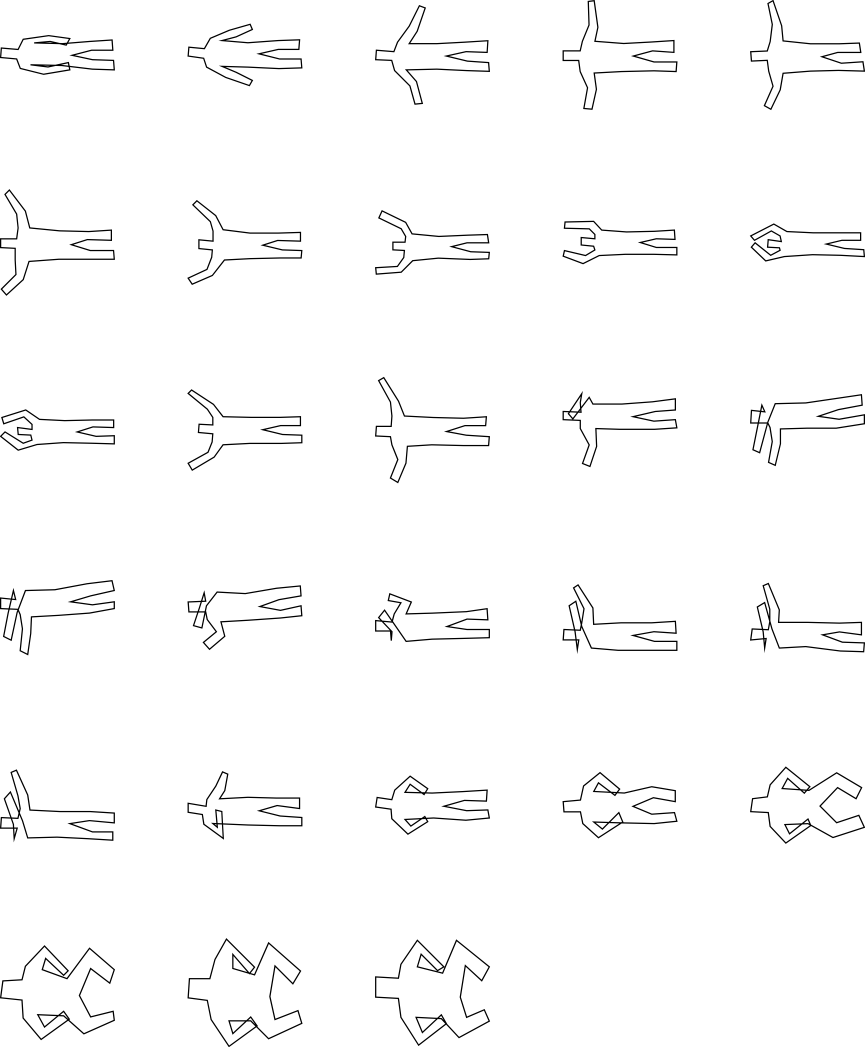
\includegraphics[width=0.5\linewidth]{experiments/3.em/multi_tuning/output.d/training.png}
\caption{Here are our training curves:}
\end{figure}

Round 10:

Here are some samples from the grammar:

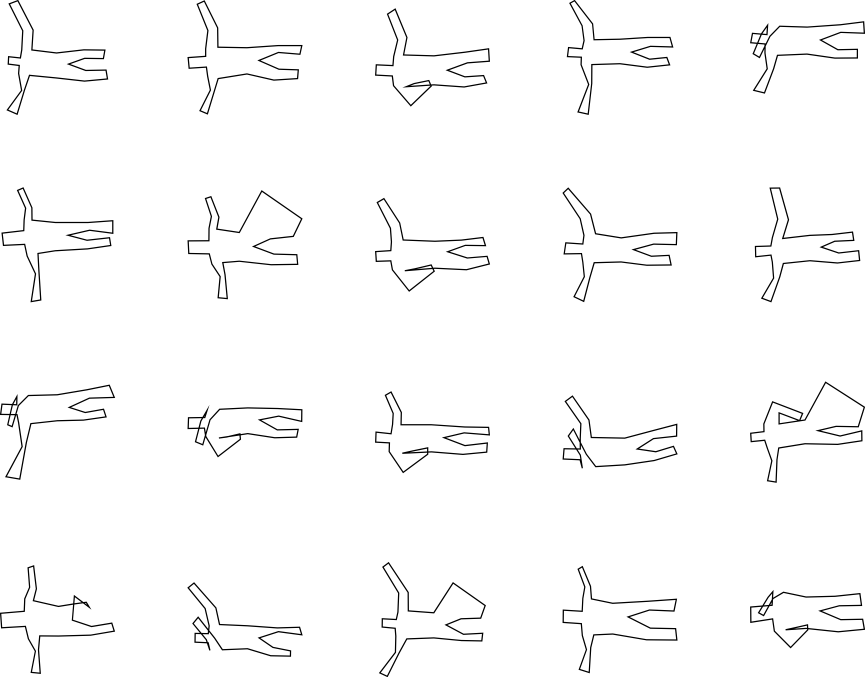
\includegraphics[width=6in]{output/3.learning/incremental/gram.19.d/samples.png}



